\begin{apendicesenv}
\partapendices

\chapter{Artigos publicados}
\label{chap:Artigo}
    A seguir os artigos publicados desde o início desta pesquisa. O primeiro artigo apresentado refere-se a publicação feita sobre este doutoramento, com resultados mistos das técnicas utilizadas na dissertação de mestrado \cite{Dissertacao} e este projeto de tese. O segundo e terceiro artigos apresentados referem-se a publicações feitas durante a dissertação, mas que expressam as técnicas utilizadas neste projeto de tese.

\section{\textit{Large-deviation quantification of boundary conditions on the Brazil nut effect}}
\label{appendix:BNE}
    This paper was published on the Physical Review E, and it is one of the main themes of this thesis, refering to chapter \ref{chap:BNE}.

\section{\textit{Methods of parallel computation applied on granular simulations}}

    Este artigo foi publicado no quatrienal do congresso \textit{Powders \& Grains 2017}, que é o maior congresso sobre materiais granulares, e que está em sua 8ª edição.

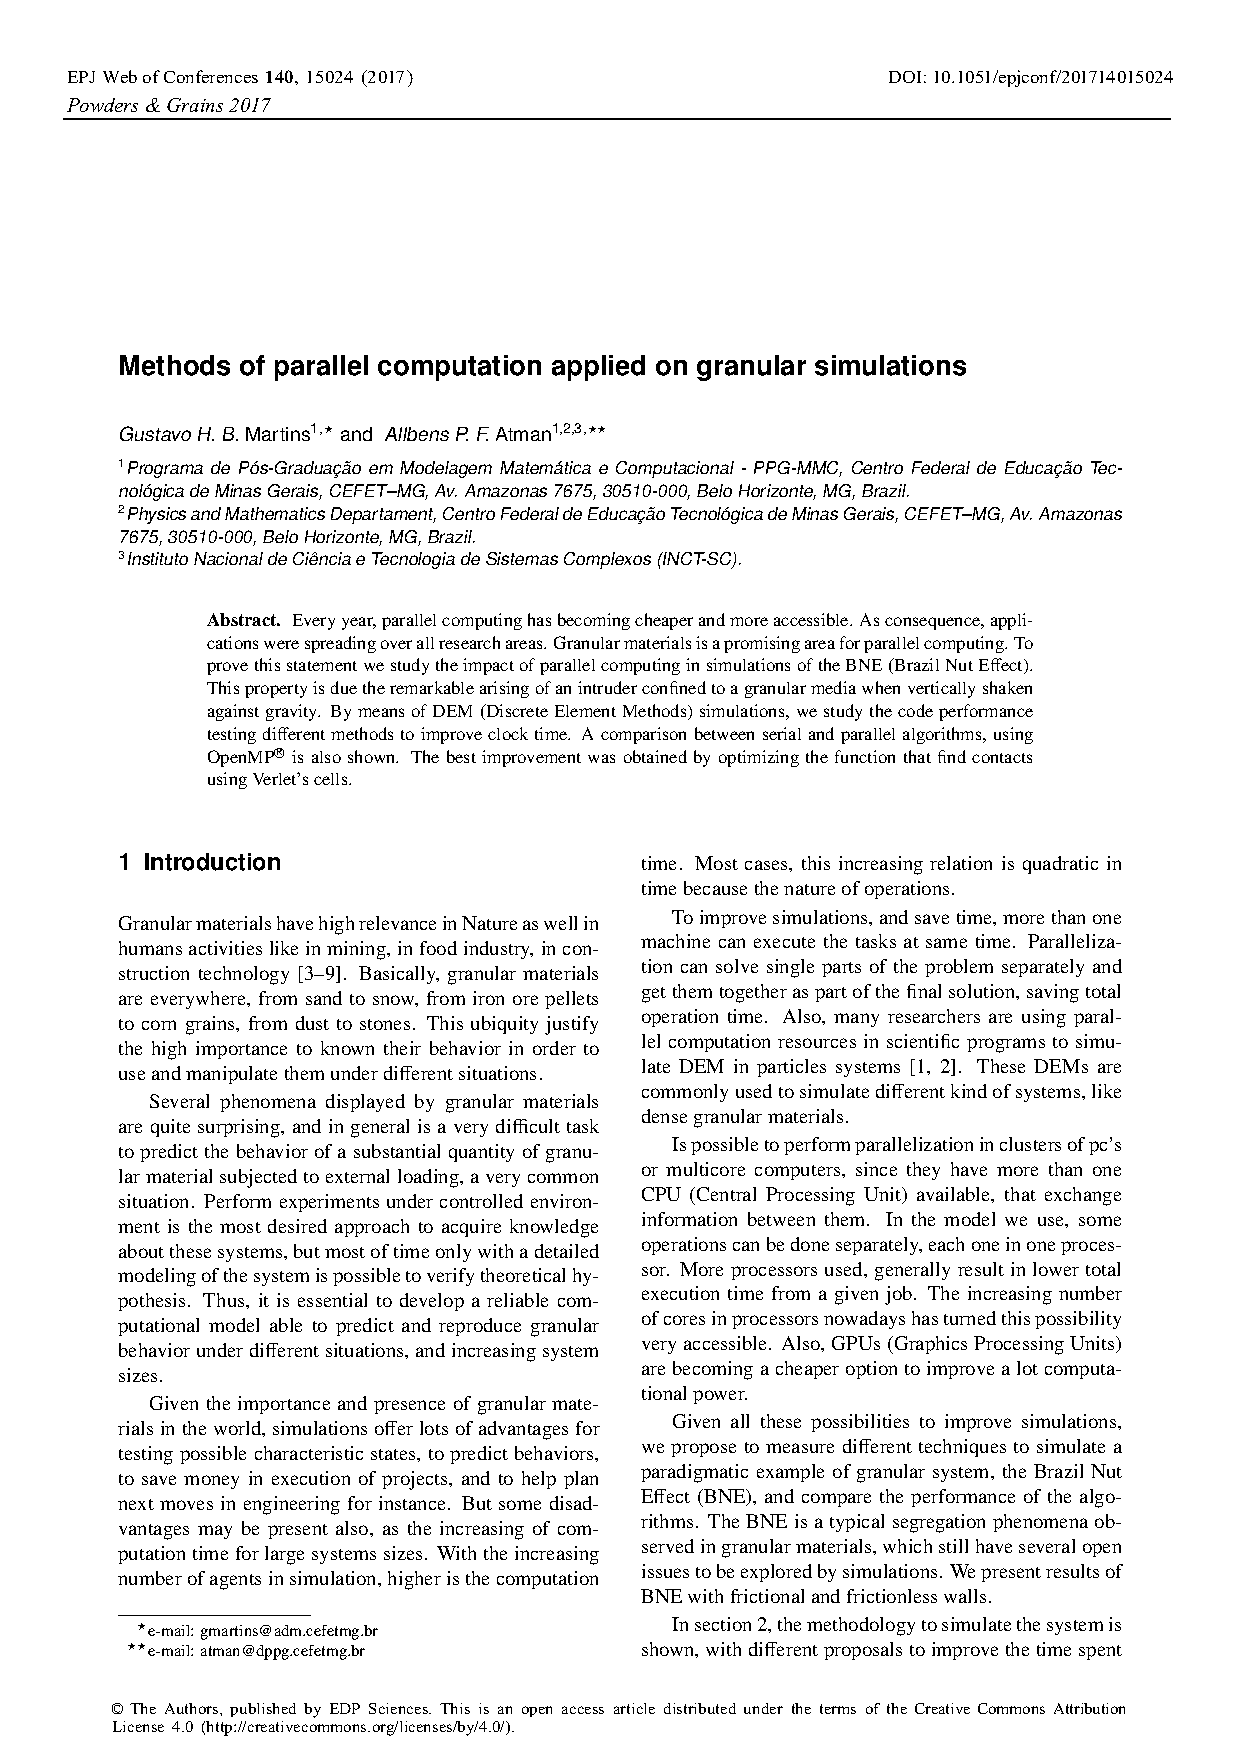
\includepdf[pages=-]{./08-apendice/ArtigoPG2017.pdf}

\section{\textit{Mechanical properties of inclined frictional granular layers}}

    Este artigo foi publicado na \textit{Granular Matter}, uma das maiores revistas sobre material granular e é uma revista A2 segundo a classificação \textit{qualis} da CAPES e possui fator de impacto de $1,762$.

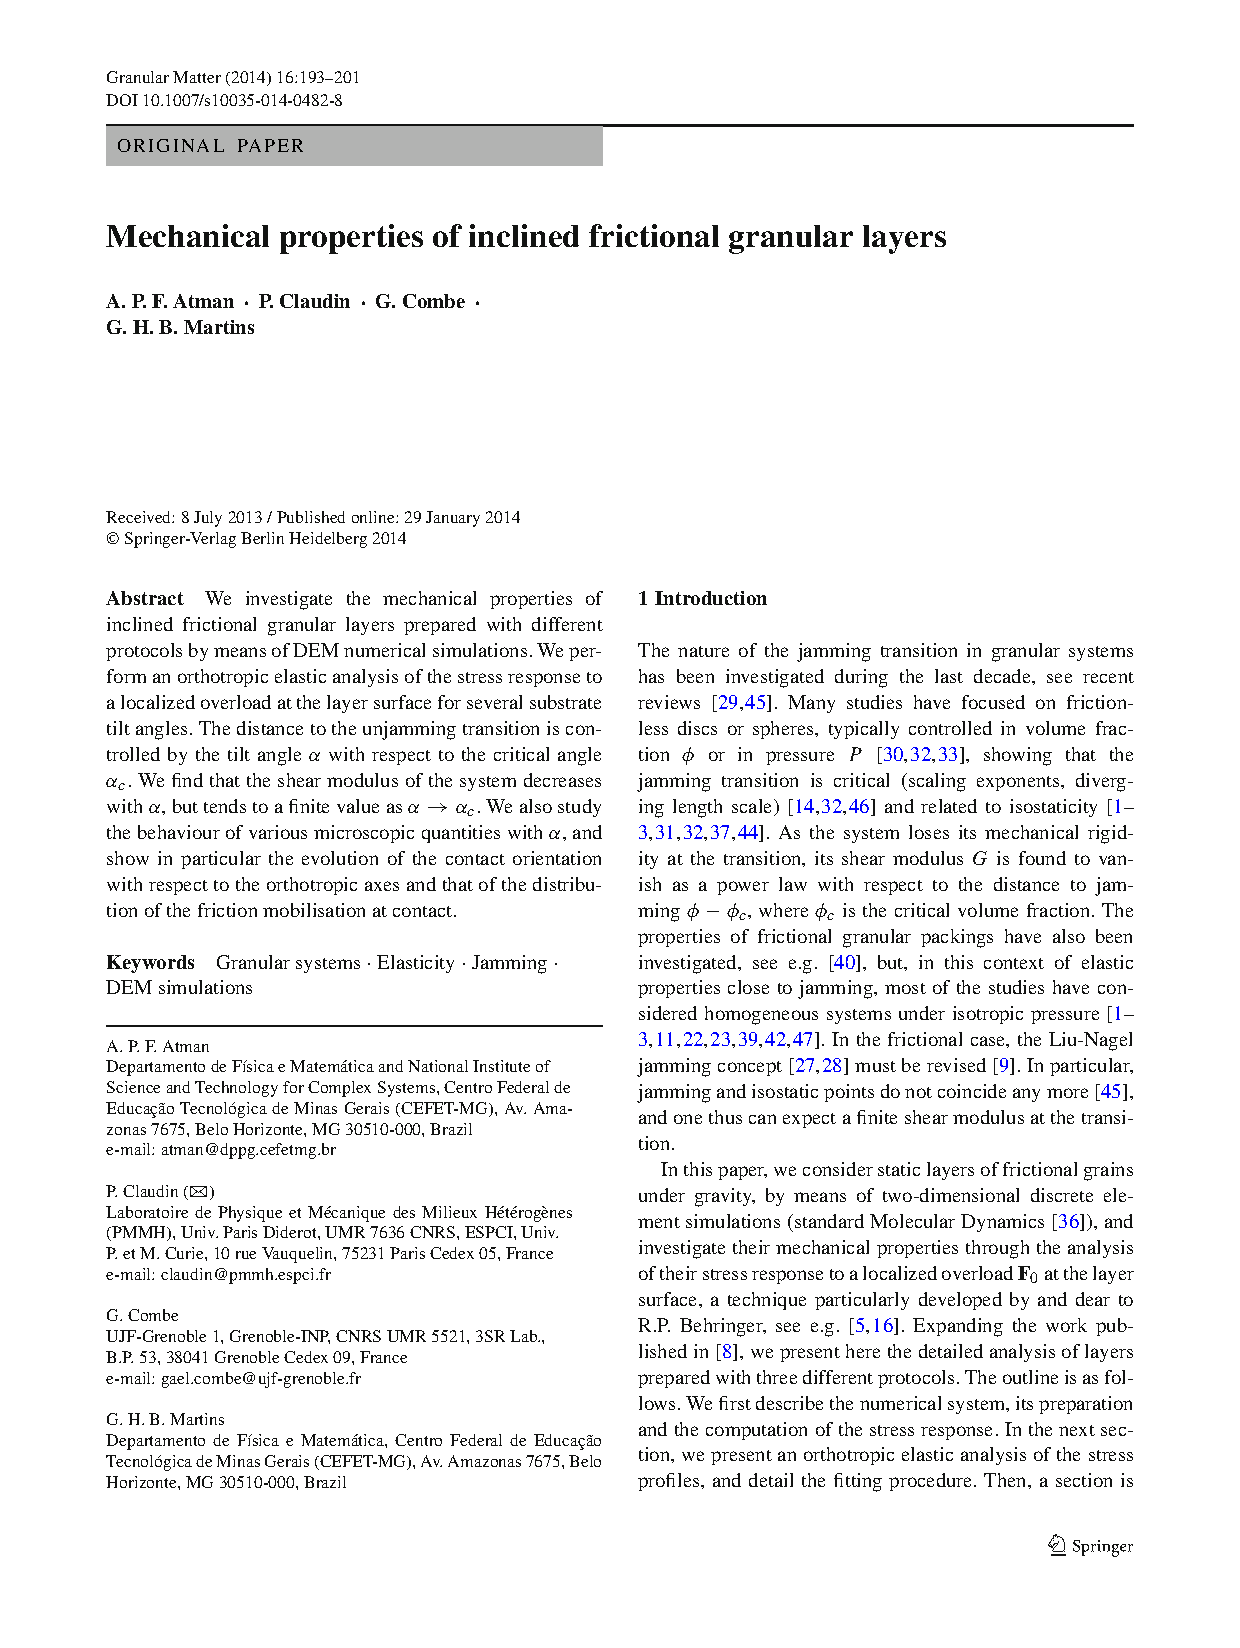
\includepdf[pages=-]{./08-apendice/ArtigoGM.pdf}

\section{\textit{Non-Gaussian behavior in jamming / unjamming transition in dense granular materials}}

    Este artigo foi publicado no quatrienal do congresso \textit{Powders \& Grains 2013}, que é o maior congresso sobre materiais granulares, e que estava em sua 7ª edição.

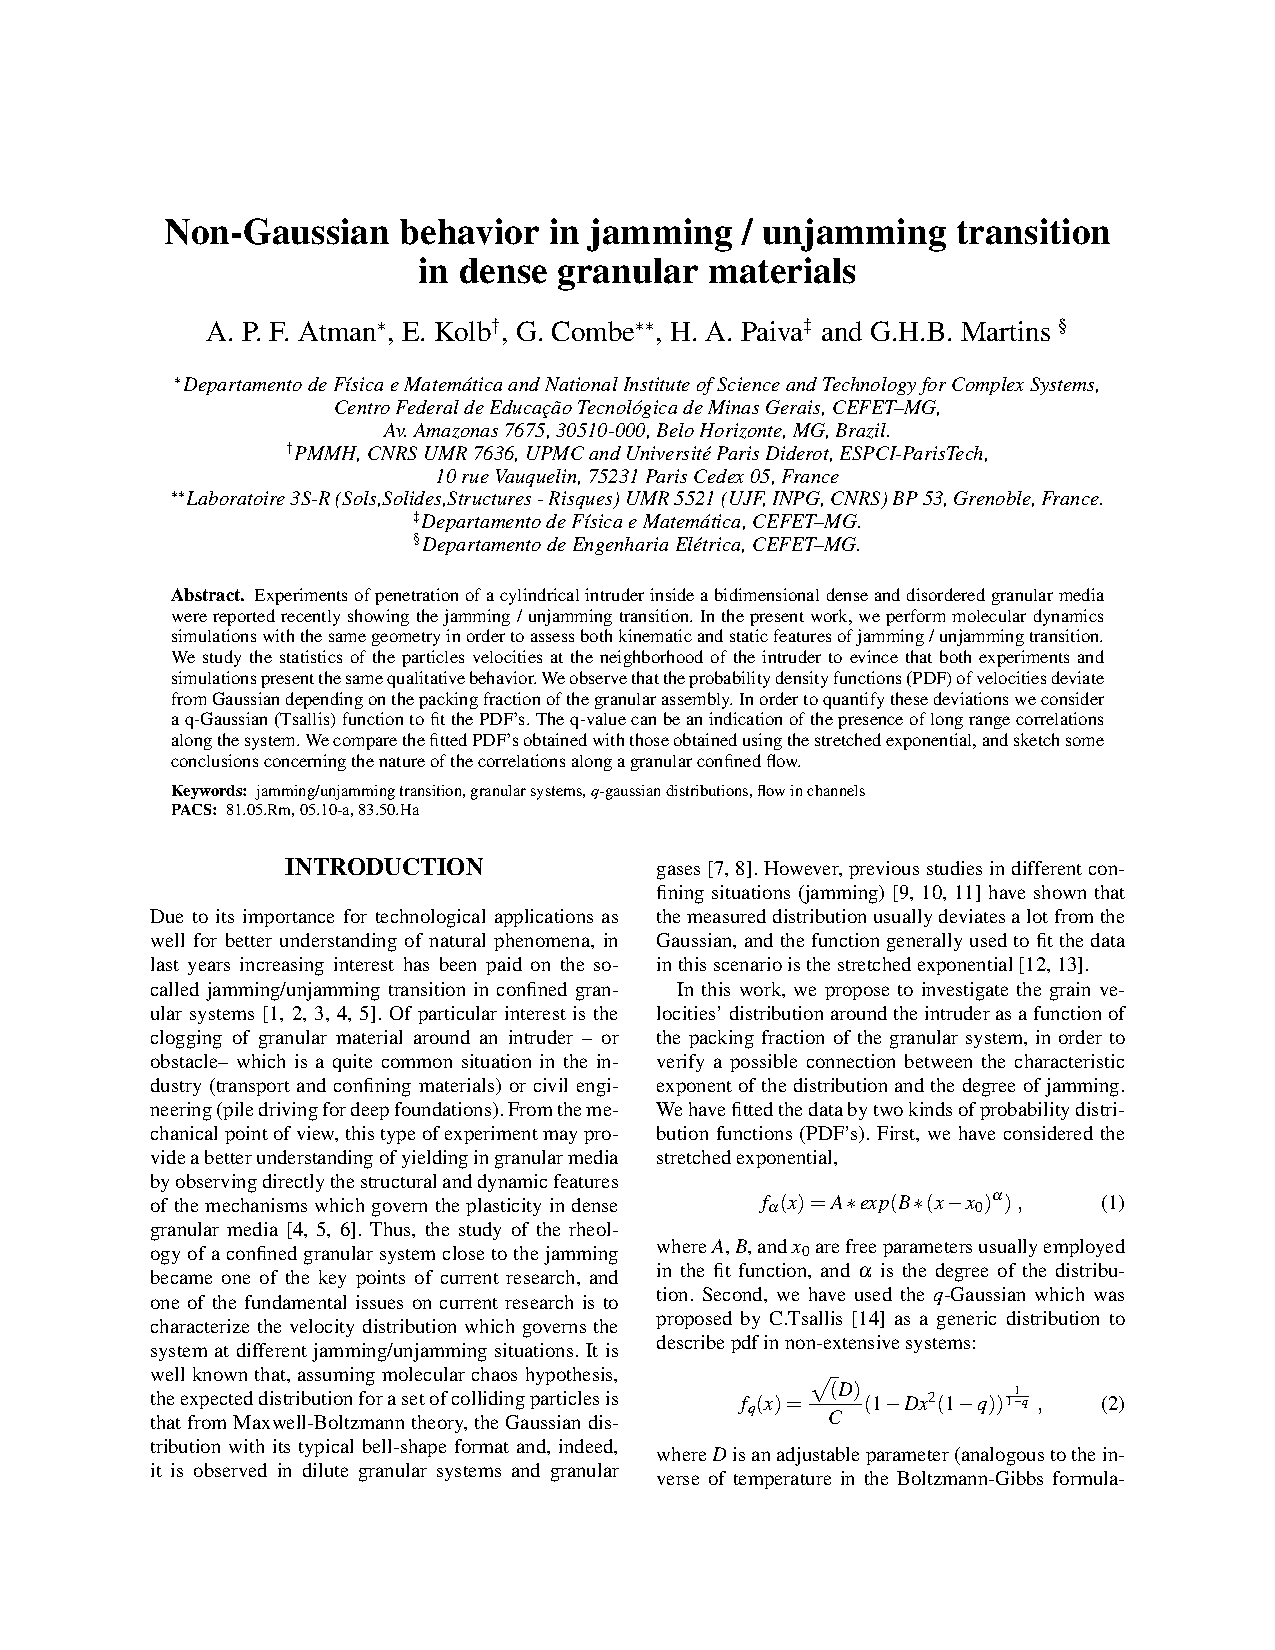
\includepdf[pages=-]{./08-apendice/ArtigoPG2013.pdf}

\chapter{Códigos}

    Coloquei os códigos utilizados para este projeto de tese em um GIT para a maior comodidade e facilidade do acesso. O endereço eletrônico é \url{https://github.com/BoscoWarhammer/Doutorado}.

\end{apendicesenv}
